\chapter{Einleitung}

% problemstellung
% ziele definieren
% vorhandene daten beschreiben
\section{Problemstellung}

\section{Benutzte Technologien}
% genutzte methoden, toolboxen, programmiersprachen
python==3.7.1 \\
numpy==1.14.2 \\
opencv-python==3.4.0.12 \\
scikit-image==0.13.1

\section{Programmaufbau}
Das Programm teilt sich in fünf Hauptkomponenten auf. Die erste ist in der \textit{main.py} zu finden, die das Programm startet und die anderen Komponenten ausführt. Die zweite Komponente kümmert sich um das entfernen des allgemeinen Hintergrunds und ist in der \textit{backgroundremover.py} zu finden. In dieser Komponente werden die eigentlichen Fotos aus dem Fotoalbum grob ausgeschnitten. Danach wird in der nächsten Komponente für jedes Foto der Rahmen der entfernt falls ein Rahmen vorhanden ist. Das entfernen des Rahmens geschieht in der \textit{rectextract.py}. Die letzte Komponente ermöglicht es Gesichter in den Ausgeschnittenen Bildern zu erkennen, dies geschieht in der \textit{facedetection.py}. Möchte man die ausgeschnittenen Bilder mit Beispielbildern vergleichen, so kann man die letzte Komponente in der Datei \textit{compare.py} verwenden. Mit deren Hilfe Metriken aufgestellt werden zum Vergleich der Bilder. In dem Flussdiagramm \ref{fig:flowchart} ist der genaue Ablauf des Programmes dargestellt. \\
\begin{figure}
	\centering
	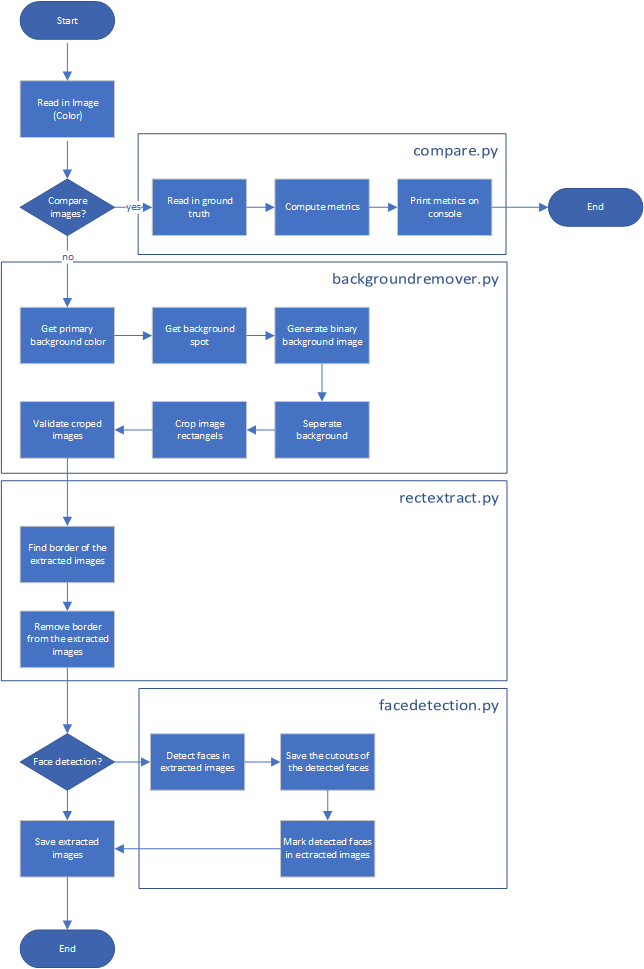
\includegraphics[width=0.8\linewidth]{images/flowchart.png}
	\caption{Flussdiagramm, das den Ablauf des Programmes darstellt. Verzweigungen können mit Hilfe von Parametern bei der Ausführung des Programmes gesteuert werden.}
	\label{fig:flowchart}
\end{figure}
